%%
%% VERSION HISTORY
%%    22 May 2006 - John Papandriopoulos - Original version
%%    12 Jul 2007 - John Papandriopoulos - Converted into template
%%

\chapter{Literature review}
	\label{chapter:a-new-hope}
	%

% preferred location for figures in this chapter
\setfigurepath{figures/chapter-2}

%=========================================================================

\iffalse
\begin{synopsis}
	In this chapter...
\end{synopsis}
\fi
%=========================================================================
\section{Types and process of suicide}
\subsection*{Types of suicide}
Suicide is defined as act of a person has self-awareness and intentionally engages in effort to end his or her life. In other word, suicidal behaviour is any active or passive acts initiated by a person with expectation to cause self-inflicted deatch. Emile Durkheim, a French sociologist specified four different types of suicide \cite{Durkheim1897}, they are illustrated in Figure~\ref{fig:types_of_suicide}.\\
\begin{figure}[!ht]
\centering
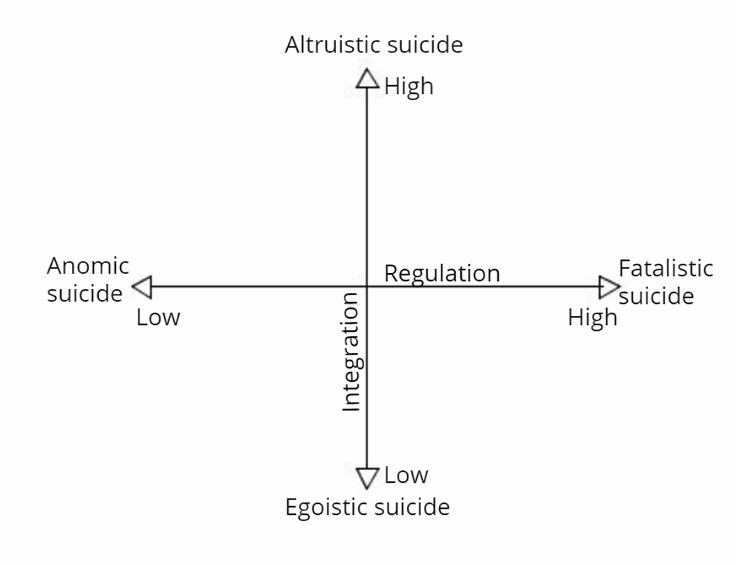
\includegraphics[width=\textwidth, clip=true]{img/type_suicide}
\caption[Types of suicide]{Types of suicide according to Émile Durkheim} 
\label{fig:types_of_suicide}
\end{figure}
(1) \textbf{Egoistic suicide:} It is a type of suicide occurs when an individual has low level of social integration. It means one does not feel he or she belong to or being accepted in a community. If this happens for a long time, it can lead to feeling of emptiness, melancholy and chronic depression. Those people feel isolated and receive little social support when they undergo hardship in life, leading to higher chance of committing suicide. It is called egoistic suicide because it springs from excessive individualism. To take example of this, Durkheim reported that the suicide rate among unmarried men is higher than that of married man since the unmarried are less bound and not connected to social norms.\\
(2) \textbf{Altruistic suicide:} In contrast to egoistic suicide, altruistic suicide occurs in societies with high integration. When an individual is overwhelmed by a community's beliefs, he put his personal values lower than community's values as a whole and considers mutual interests of community is more important than his needs. Examples for this type of suicide are suicide bomber and Samurai from Japan. Suicide bombers believe their death contribute to progress of his group to a common goal. In Samurai's code of feudal Japan, a Samurai who fail to complete an assigned task or lose in battle is seen as disgrace thus a samurai commits suicide when he feels humiliation and dishonored.\\
(3) \textbf{Anomic suicide:} Anomic suicide takes place in society with low degree of regulation. In a situation of sudden economic and social turmoil, an individual may question his morality due to lacking of social direction and deregulation of social ethic. People get frustrated when they fail to realize their desires and are being disappointed by it constantly. An example of this is suicide rate surges when there is a economic upheaval, crash of stock market or bankruptcy.\\
(4) \textbf{Fatalistic suicide:} Opposite to anomic suicide, fatalistic suicide happens when people are kept under tight regulation. An overregulated society has extreme rules and discipline, making its inhabitants feel suffocated by high standard and expectation. These people would prefer death to living within such harsh environment. Typical example of this kind of suicide is students under pressure of academic performance set by parents or their teachers.\\

\subsection*{Process of suicide}
According to authors of \cite{O'Carroll1996}, suicide ideation refers to an individual's rumination about conducting suicidal behaviour. Suicide plan includes idea about time, location and method of suicide. Suicide attempt is a self-initiated, self-inflicted and injurious act following suicide plan performed in order to end one's life.\\
Figure~\ref{fig:suicide_process} shows the process of suicide. Suicide ideation is first phase, where thought of suicide appear with possibly a statement or threat of suicide. Suicide plan precedes actual suicide attempt, it is characterized by suicide rehearsal which is behavioral enactment of a lethal method for suicide.\\
It is important to identify suicide ideation because taking action early may stop progression of suicide process. Therefore, spotting suicide ideation is vital and should be top priority in suicide prevention.
 
\begin{figure}[!ht]
\centering
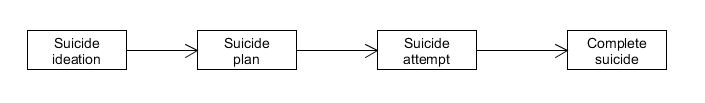
\includegraphics[width=\textwidth, clip=true]{img/suicide_process}
\caption[Process of suicide]{Flow diagram of suicide process} 
\label{fig:suicide_process}
\end{figure}

\section{Emotion classification in suicide notes}
Although the research of suicidal text started in 1960s with linguistic analysis of suicide notes to distinguish between genuine and stimulated notes, the application of natural language processing  and machine learning in the same task appear in 2010 \cite{Desmet2013}. Pestian et al \cite{Pestian2010} applied ML algorithms to differentiate the notes of suicide completer and notes written by healthy control group and compared the accuracy of classifiers to accuracy of mental health providers. The best algorithm obtained the accuracy of 78\%, exceeding human professionals accuracy by 13\%. This promising result laid the foundation of NLP techniques on suicide notes. It also suggests the potential possibility of computer assist human in assessing suicide risk. However, the sample size for the study is only 66 and is derived from old study which reduce the reliability since the machine focus on the structure of the notes rather than content like what human usually do. Previously, Huang et al \cite{Huang2008} collected blog entries from MySpace.com and use dictionaries containing suicide-related keywords to detect blogs with suicidal intention. The study is one of the first to use social media data to find suicide thoughts and that, in turn, set the new goal for NLP in the mental research: identifying mental suffering victims actively using social network and are at brink of suicide. Unfortunately, MySpace lost its popularity lead to researchers switching to other social networking sites for their study and finding the keyword is a primitive approach for a NLP task.\\

In 2011, the competition i2b2 NLP Challenge\footnote{https://www.i2b2.org/NLP/Coreference/} attracted 106 scientists from 24 teams to solve a shared task \cite{Pestian2012}. Track 2 of the challenge require participants to classify sentences in suicide notes in one or more of 15 categories which are 13 emotions such as love, guilt and 2 nonemotion class namely instruction and information. The training set is 600 actual suicide notes collected by Dr. Edwin Shneidman and Cincinnati Children Hospital Medical Center and annotated by different reviewers. Each team is allowed to submit at most three systems thus some teams have similar strategies: develop two classifiers and "combine" them into a hybrid classifier. Wang et al \cite{Wang2012} developed a ML classifier using support vector machine (SVM) along with "one-against-one" approach for multi-label classification. Before training the data, they pre-processed data to aim for betting parser accuracy and give similar meaning to syntactically different expression. For example, they correct misspellings, normalize symbol and number (’+’ to ’and’, ’\$100’ to ’\$MONEY\$’). Their second system is a rule-based classifier that create set of patterns from training data automatically and using $\chi^2$ test and choose a fixed number of pattern set to reduce pattern space. A notion called g-measure was defined, it is a conditional probability of sentence that contain a specific pattern belong to a specific class. The highest g-measure is chosen for that categories to be labelled for a sentence if it is higher than a specific threshold. The team has experimented to find threshold that produce highest F-score and choose it to be fixed threshold for hybrid system. A simple combination rule is used to form a hybrid classifier: if a sentence is not labelled by SVM classifier, then result of rule-based classifier is assigned to that sentence. The threshold approach gives better precision (often higher than 0.6) than recall (lower than 0.4) since there are some sentences with various emotions in them and the threshold overlook low occurrence emotion.\\

Similarly, Sohn et al \cite{Sohn2012} proposed a ML system and a rule emphasis system. They used Weka (Waikato Environment for Knowledge Analysis \footnote{https://www.cs.waikato.ac.nz/ml/weka/}) and its multinomial Naive Bayes to create the ML system. Some techniques are applied in the process namely token normalization (e.g. "can’t", "ca n’t" convert to "cannot"), classifier ensemble (using different values for a parameter) and corpus-reannotation. Their rule-based system simply utilizes Perl regular expressions to match defined patterns. Again, hybrid system combines the result of the two systems to get the final label. They have more balanced result between precision and recall with both are in range 0.5 to 0.6. They also have data pre-processing with popular methods like symbol normalization using regular expression and post-processing phase. A shortcoming of this paper is lack of deep syntactic analysis making some rare classes (sorrow, forgiveness, abuse) did not occur at all. Another improvement can be made by analyze the effect of combining two systems, why it only improves the F-score just a tiny bit compared to other systems.\\

Luyckx et al \cite{Luyckx2012} approached the problem with a new way as they pre-process the data then carry out two processing phases: calibration and thresholding. In the pre-processing step, they tried to divided multi-labelled sentences into single-labelled fragments. If the sentence cannot be divided, then it would be discarded from training data. The calibration phase use SVM classifier with ten-fold cross-validation scheme on output of pre-processing step and evaluate lexical features, context features and lexicon-based features. The lexical features include some frequently occurred word that associated with a specific emotion (e.g. "can’t", "tired" for hopelessness). The context features consider the label of preceding and following sentences while lexicon-based features make use of a vocabulary of emotion. The thresholding phase applied various threshold to LibSVM (a learning package) probability estimates. In term of F-score, out of these three group, Union system of Sohn’s group attained highest score of 0.5640 followed by 0.5038 and 0.5018 of Wang’s team and Luyckx’s team respectively. The mean performance of all team is 0.4875 with the median of 0.5027. The team with highest score achieve F-measure of 0.6139. The differences between these systems are summarized in Table~\ref{tab:teams}.\\

\iffalse

\begin{table}[]
\centering
\caption{My caption}
\label{my-label}
\begin{tabular}{lllll}
\hline

                    & Microaverage F1  &   Multi-system                              &  Learning algorithm            &   Feature engineering\\ \cline{2-5} 
Sohn's team &  0.5640                & Yes (ML, rule-based and hybrid) &  Multinomial naive Bayes    &  Named Entity Recognition, n-gram tokenization, token normalization \\
Wang's team&  0.5038                & Yes (ML, rule-based and hybrid) & one-against-one SVM        &   n-gram tokenization, POS tagging, sentiment analysis\\
Luyckx's team&  0.5018              & No                                                & one-vs-all SVM                   & Multi-label training sentences re-annotated into single-label instances, unigram tokenization  \\ \hline
\end{tabular}
\end{table}
\fi
\begin{table}
\noindent\begin{tabularx}{\textwidth}{llXXX}

\toprule
                    & Micro-average F1  &   Multi-system                              &  Learning algorithm            &   Feature engineering\\ 
\midrule
Sohn's team &  0.5640                & Yes (ML, rule-based and hybrid) &  Multinomial naive Bayes    &  Named Entity Recognition, n-gram tokenization, token normalization \\
Wang's team&  0.5038                & Yes (ML, rule-based and hybrid) & one-against-one SVM        &   n-gram tokenization, POS tagging, sentiment analysis\\
Luyckx's team&  0.5018              & No                                                & one-vs-all SVM                   & Multi-label training sentences re-annotated into single-label instances, unigram tokenization\\	

\bottomrule
\end{tabularx}
\caption{Comparison between teams: each team take different approaches, learning algorithm and feature engineering method}
\label{tab:teams}
\end{table}


Although all three teams have done some pre-processing steps but only Sohn’s team do post-processing part to eliminate misclassified cases such as salutation being labelled instruction. They also used different learning algorithm from other teams (Naive Bayes vs SVM). This can be one of the reasons why they have smaller difference between precision and recall compared to their counterpart. Naive Bayes is usually work well on small tex collection. Unfortunately, Luyckx’s team could have achieved better result if they did not re-annotate the data. They chose to re-annotate because it show promising result in the development phase but it turn out not good as they expect with F-score of 0.5018 while intact data could give them 0.5230 with roughly the same precision and recall (0.53 and 0.5 respectively). In these papers, the teams use stadard, well-known methods in NLP and off-the-shelf packages to implement their systems, and it is not surprise since this challenge aim is to apply techniques to problem, not investigating pure theory.


\section{Analysis of suicide on social media}
Another research trend is using social media data to relate blog posts and suicide cases. Won et al \cite{Won2013} build a model to predict to suicide number in South Korea. Their model considers social media data in form of suicide and dysphoria weblog (blog entries containing specific words relate to suicide or dissatisfaction with one’s life), economic and meteorological data which are Korea Composite Stock Price Index (KOSPI) and temperature. Another interesting features is celebrity suicides are also have quite strong correlation with number of suicide in that month. At the same time in the USA, Jashinsky et al \cite{Jashinsky2014}  investigated the suicide risk factors via Twitter data. They collected tweet (small blog entry with 140 characters restriction) with Twitter application programming interface (API). The API allow users to retrieve tweet in a specific period of time with some available criteria such as keyword. They created a list of filter term to identify high concerning entries and attempted to remove the entries with joke, sacarstic intention. The result shows there is correlation between observed Twitter data with data obtained from real world suicides in states with highest suicide rate such as Alaska, New Mexico and Idaho. Both studies focus on public blogs containing keywords and actual suicide number but there are differences between them: sample data duration range (3 months vs 3 years), geolocation (each states vs whole nation), number of variables. These studies suggest it is good idea to incorporate social media data into model that inspect suicide trend across geographic regions but more filter must be developed to get messages of real victim rather than relying on keywords in blog.


